\documentclass{article} % For LaTeX2e
\usepackage{nips14submit_e,times}
\usepackage{cite}
\usepackage{enumitem}
\usepackage{algorithm,algorithmicx}
\usepackage[noend]{algpseudocode}
\usepackage{url,graphicx,amsmath}
\usepackage{caption}
\usepackage[caption=false]{subfig}
%\documentstyle[nips14submit_09,times,art10]{article} % For LaTeX 2.09
\usepackage[pagebackref=true,breaklinks=true,letterpaper=true,colorlinks,bookmarks=false]{hyperref}

\title{Recruitment Analytics: Predict Applicant Behavior from Sparsely Labeled }

\author{
%XIN LIN \\
%Department of Computer Science\\
%University of Texas at Austin \\
%Austin, TX 78705 \\
%\texttt{jimmylin@utexas.edu} \\
%\And
%Coauthor \\
%Affiliation \\
%Address \\
%\texttt{email} \\
%\AND
%Coauthor \\
%Affiliation \\
%Address \\
%\texttt{email} \\
%\And
%Coauthor \\
%Affiliation \\
%Address \\
%\texttt{email} \\
%\And
%Coauthor \\
%Affiliation \\
%Address \\
%\texttt{email} \\
%(if needed)\\
}

% The \author macro works with any number of authors. There are two commands
% used to separate the names and addresses of multiple authors: \And and \AND.
%
% Using \And between authors leaves it to \LaTeX{} to determine where to break
% the lines. Using \AND forces a linebreak at that point. So, if \LaTeX{}
% puts 3 of 4 authors names on the first line, and the last on the second
% line, try using \AND instead of \And before the third author name.

\newtheorem{remark}{Remark}
\newcommand{\fix}{\marginpar{FIX}}
\newcommand{\new}{\marginpar{NEW}}

\nipsfinalcopy % Uncomment for camera-ready version

\begin{document}


\maketitle

\section{Introduction}

\section{Formulation}
\subsection{Optimization}
\subsubsection{Classic Matrix Completion}
% 2.2 latent factor model 
The latent factor model has an underlying assumption: the real exact rating matrix are
low-rank matrix. By modelling target rating variable as 
\begin{align}
    R_{ij} = U_i^T V_j 
\end{align}
Then we are able to use least square cost to guide the optimization procedure: 
\begin{equation}
    \begin{aligned}
        &\min_{U,V} 
        && \sum_{(i,j)} (A_{ij} - U_i^T V_j)^2
        + \frac{\lambda}{2}(||U||_F^2 + ||V||_F^2)
    \end{aligned}
\end{equation}
where $A_{i,j}$ is the observed ground-truth entry and $\Omega$ is the index set of
entries that are observed. 

\subsubsection{One-Class Matrix Completion}
\begin{equation}
    \begin{aligned}
        &\min_{U,V} 
        && \sum_{(i,j)\in \Omega} (1 - U_i^T V_j)^2
        + \frac{\lambda}{2}(||U||_F^2 + ||V||_F^2)
    \end{aligned}
\end{equation}
%\begin{remark}
%    Since some jobs have fairly limited number of previous history, then
%    One-Class Matrix Completion is expected to have bad performance.
%\end{remark}
\subsubsection{Inductive Matrix Completion}
% brief math introduction
Formulate the problem as that of recovering a low-rank matrix $W_*$ using
observed entries $R_{ij} = x_i^T W_{*} y_j$ and the user/job feature vectors $x_i$, $y_j$. By
factoring $W = U V^T$ , we see that this scheme constitutes a bi-linear
prediction $(x^T U_{*})(V_{*} y)$ for a new user/job pair $(x, y)$.
\begin{equation}
    \begin{aligned}
        &\min_{U,V} &&\sum_{(i,j)} (A_{ij} - x_i^TUV^Ty_j)^2 
        + \frac{\lambda}{2}(||U||_F^2 + ||V||_F^2)
    \end{aligned}
\end{equation}
% break through: dhillon's paper - inductive matrix completion
According to \cite{jain2013provable}, under standard set of assumptions,
the alternating minimization provably converges at a linear rate to the global
optimum of two low-rank estimation problems: a) RIP measurements based general
low-rank matrix sensing, and b) low-rank matrix completion. A more recent
paper \cite{natarajan2014inductive} in bioinformatics demonstrated successful
application of such inductive matrix completion
framework on gene-disease analytics.

\subsubsection{One-Class Inductive Matrix Completion}
\begin{equation}
    \begin{aligned}
        &\min_{U,V} &&\sum_{(i,j)\in\Omega} (1 - x_i^TUV^Ty_j)^2 
        + \frac{\lambda}{2}(||U||_F^2 + ||V||_F^2)
    \end{aligned}
\end{equation}

\subsubsection{One-Class Inductive Matrix Completion with Biases}
\begin{equation}
    \begin{aligned}
        &\min_{U,V} &&(1-\alpha) \sum_{A_{ij}=1} (1 - x_i^TUV^Ty_j)^2 +
        \alpha \sum_{A_{ij}=0} (0 - x_i^TUV^Ty_j)^2 + \frac{\lambda}{2}(||U||_F^2 + ||V||_F^2)
    \end{aligned}
\end{equation}

%\subsection{One-Class Inductive Matrix Completion with kernel method}
%% 3.2 propose kernel-based inductive matrix completion?
%One possible enhancement for above inductive matrix completion is to
%extend our consideration from the linear association between features and
%latent factors to an version that accepts non-linear association.
%By this intuition, we can name this approach as 
%    {\it Kernel-based Inductive Matrix Completion}.
%By taking into account non-linear relations between designed features and hidden
%topics (shared latent factors), the space of latent factors can be largely
%expanded and then it would be more likely to automatically detect latent
%factors with higher quality. 
% 
%\subsection{One-Class Inductive Matrix Completion with pre-clustering}
\subsection{Assessments}
In this research project, we employ Recall-Precision curve and MAP@N curve to 
asess and visually present the accurate performance of a particular model. 
\subsubsection{Recall-Precision Curve}
% precision and recall definition
In pattern recognition and information retrieval with binary classification,
precision, a.k.a. positive predictive value, is the fraction of retrieved
instances that are relevant, while recall, a.k.a. sensitivity, is the
fraction of relevant instances that are retrieved. According to the general
definition, the precision and recall in this recommendation problem can be
formulated as 
\begin{align}
    \text{precision} &=  \\
    \text{recall} &= 
\end{align}
% TODO: advantage of rp curve

% weakness of rp curve
Nevertheless, precision and recall are single-value metrics that take no ordering information
into account. Thus, the recall-precision curve cannot assess performance of a
model from the "order-does-matter" perspective.
\subsubsection{MAP@N Curve}
For job recommendation system, it is supposed to return a ranked sequence of
suitable jobs for users to apply. Therefore, it is desirable to also consider the
order in which the returned jobs are presented. The mean average precision
(MAP) does vary in terms of the order of returned jobs and thus cumulative
MAP@N curve can serve as an effective tool to visualize the quality of queried
recommendations for both ordering and accuracy.

% AP
The prerequisite of computing mean average precision is to figure out average
precision (AP) for each queried user. The average precision at certain
position $N$ is defined as
\begin{align}
    \text{AP@N} &= 
\end{align}

% MAP
Taking the mean of average precision at the corresponding position for all
queried users derives the mean average precision .
\begin{align}
    \text{MAP@N} &= 
\end{align}

% MAP@N remark

\section{Implementation}
\subsection{Algorithm}
% algorithm presentation
\newcommand{\xii}{\boldsymbol{x}_i}
\newcommand{\yj}{\boldsymbol{y}_j}
The algorithmic description for {\it One-class Inductive Matrix Completion
    with biased weight} are shown in Algorithm \ref{alg:AltMin}.  
\begin{algorithm}
    \caption{Alternating Minimization for One-Class Inductive Matrix Completion with Biases}
    \label{alg:AltMin}
    \begin{algorithmic}[1]

\State \textbf{INPUT}: \\ \ \ a) sparse matrices $X$ and $Y$ that denote features of users
and jobs respectively. \\ \ \ b) matrix $A$ that denotes partial observation
of "apply" association with observed index set $\Omega$ \State \

\State Initialize $U_{(0)}$ and $V_{0}$ by uniform randomization
\State \textbf{Do}  
\State \ \ \
$V_{(k+1)}$ = argmin $(1-\alpha) \sum_{(i,j) \in \Omega} 
    (1- \xii^T U_{(k)} V_{(k)}^T \yj)^2 
    + \alpha \sum_{(i,j) \not \in \Omega} (0 - \xii^T U_{(k)} V_{(k)}^T \yj)^2$

\State \  \
$U_{(k+1)}$ = argmin $(1-\alpha) \sum_{(i,j) \in \Omega}
    (1-\xii^T U_{(k)} V_{(k+1)}^T \yj)^2 +
    \alpha \sum_{(i,j) \not \in \Omega}
    (0-\xii^T U_{(k)} V_{(k+1)}^T \yj)^2$
\State \textbf{Until} Convergence. 
%\State Predict values for missing entries: for some $ (i,j) \not \in \Omega$,
%\State 
%\ \  \ $R_{ij} = 1,\ \text{for top } r $ items
%\State 
%\ \  \ $R_{ij} = 0,\ \text{otherwise}$

\State \

\State \textbf{OUTPUT: } \\ 
\ \ a) Model Parameter $ U_{*}$ and $V_{*}$ 
\end{algorithmic}
\end{algorithm}

%{{{ Newton Conjugate descent Method
\begin{algorithm}
    \caption{Newton Conjugate Descent Subroutine}
    \label{alg:newton}
    \begin{algorithmic}[1]

\State \textbf{INPUT}: \\ \ \ a) 
\\ \ \ b) 
\State \

\State Initialize $U_{(0)}$ and $V_{0}$ by uniform randomization
\State \

\State \textbf{OUTPUT: } \\ 
\ \ a) Model Parameter $ U_{*}$ and $V_{*}$ 
\end{algorithmic}
\end{algorithm}
%}}}

%{{{ Prediction Routine
\begin{algorithm}
    \caption{Prediction}
    \label{alg:prec}
    \begin{algorithmic}[1]

\State \textbf{INPUT}: \\ \ \ a) sparse matrices $X$ and $Y$ denote features of users
and jobs. \\ \ \ b) matrix $A$ denotes partial observation of application
association with observed index set $\Omega$
\State \

\State Initialize $U_{(0)}$ and $V_{0}$ by uniform randomization
\State \

\State \textbf{OUTPUT: } \\ 
\ \ a) Model Parameter $ U_{*}$ and $V_{*}$ 
\end{algorithmic}
\end{algorithm}
%}}}

%{{{ Preclustering
\begin{algorithm}
    \caption{Preclustering}
    \label{alg:preclustering}
    \begin{algorithmic}[1]

\State \textbf{INPUT}: \\ \ \ a) sparse matrices $X$ and $Y$ that denote features of users
and jobs respectively. \\ \ \ b) matrix $A$ that denotes partial observation
of "apply" association with observed index set $\Omega$ \State \

\State Initialize $U_{(0)}$ and $V_{0}$ by uniform randomization
\State \textbf{Do}  
\State \ \ \
$V_{(k+1)}$ = argmin $(1-\alpha) \sum_{(i,j) \in \Omega} 
    (1- \xii^T U_{(k)} V_{(k)}^T \yj)^2 
    + \alpha \sum_{(i,j) \not \in \Omega} (0 - \xii^T U_{(k)} V_{(k)}^T \yj)^2$

\State \  \
$U_{(k+1)}$ = argmin $(1-\alpha) \sum_{(i,j) \in \Omega}
    (1-\xii^T U_{(k)} V_{(k+1)}^T \yj)^2 +
    \alpha \sum_{(i,j) \not \in \Omega}
    (0-\xii^T U_{(k)} V_{(k+1)}^T \yj)^2$
\State \textbf{Until} Convergence. 
%\State Predict values for missing entries: for some $ (i,j) \not \in \Omega$,
%\State 
%\ \  \ $R_{ij} = 1,\ \text{for top } r $ items
%\State 
%\ \  \ $R_{ij} = 0,\ \text{otherwise}$

\State \

\State \textbf{OUTPUT: } \\ 
\ \ a) Model Parameter $ U_{*}$ and $V_{*}$ 
\end{algorithmic}
\end{algorithm}
%}}}


\subsection{Practical Issues}
\textbf{Bias}. Bias parameter $\alpha \in (0, 1)$ is the weight to balance
optimization objective between observed and missing labels. Note that we can
simply set $\alpha = 1$ to solve unbiased version of one-class inductive matrix completion.

\textbf{Initialization}. Randomizing all components of $U_{(0)}$ and
$V_{(0)}$ to uniform distribution over $(0, 1)$ works well in our
experimentation. 

\textbf{Optimization}.
During each stage of alternating minimization, standarded conjugate gradient method is
employed to solve least square problem. 

\section{Experiment I: Feature Extraction} % 3 pages
\subsection{Dataset} 

\subsection{Preprocessing}

\section{Experiment II: Basic Parameters} % 4 pages

\subsection{Effects of Rank $K$}
We trace the main term in training stage.
\begin{figure}[hp]
    \centering
    \captionsetup{justification=centering}
    \subfloat{ 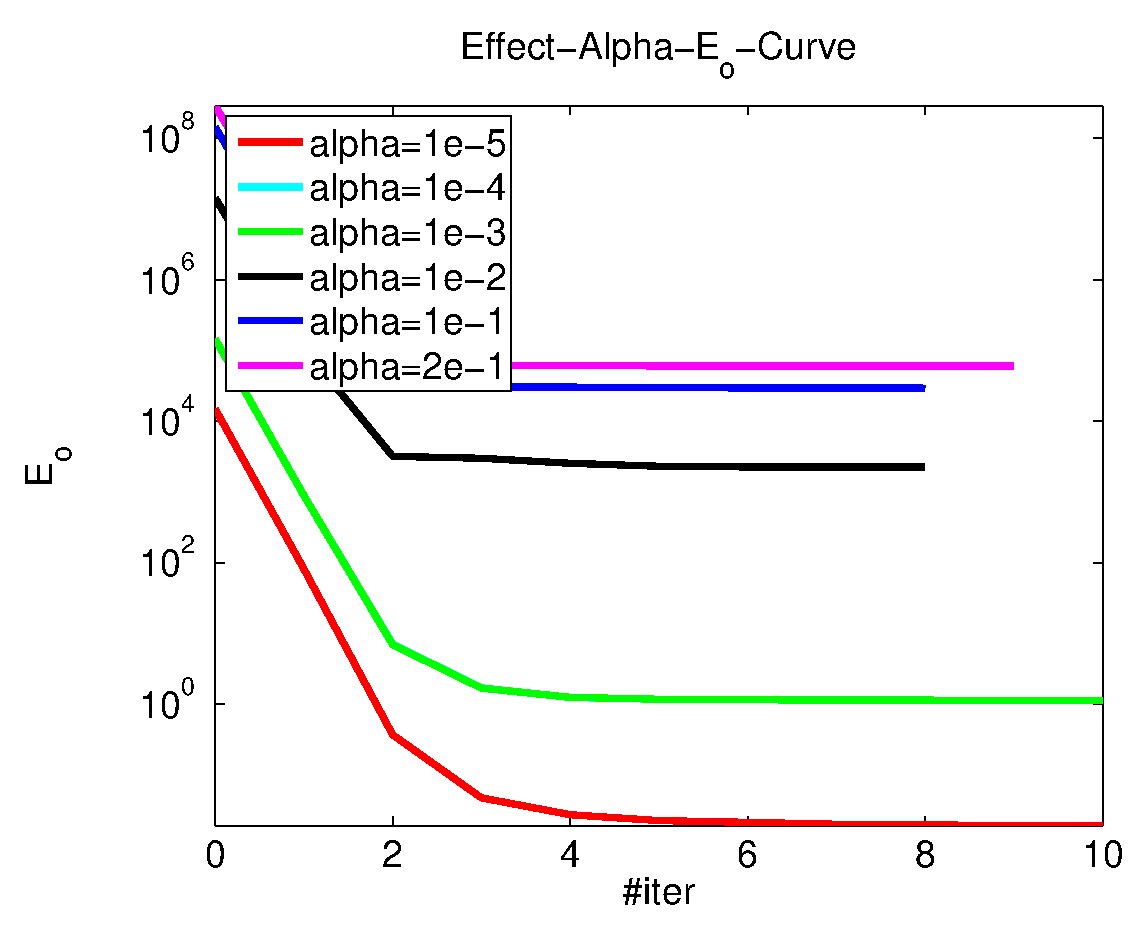
\includegraphics[width=65mm]{Effect_K/E_o_Curve.eps} }
    \subfloat{ 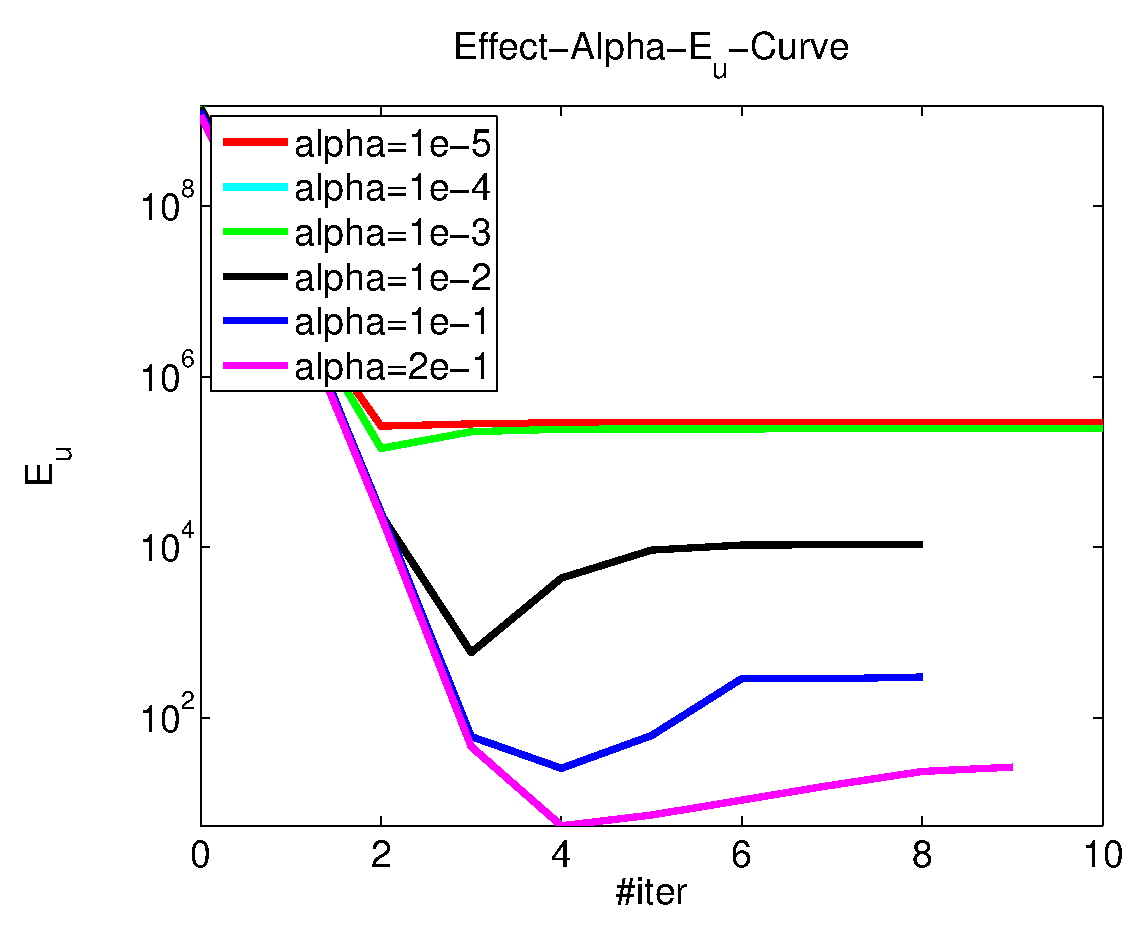
\includegraphics[width=65mm]{Effect_K/E_u_Curve.eps} }
    \caption{Trace $E_o$ and $E_u$ between the trained models with various
        $K=5,10,20,30,50$. \newline
        Left: $E_o$ Curve. Right: $E_u$ Curve. } 
    \label{EffectK:Eo_Eu}
\end{figure}

The performance evaluation is as follows.
\begin{figure}[hp]
    \centering
    \captionsetup{justification=centering}
    \subfloat{
        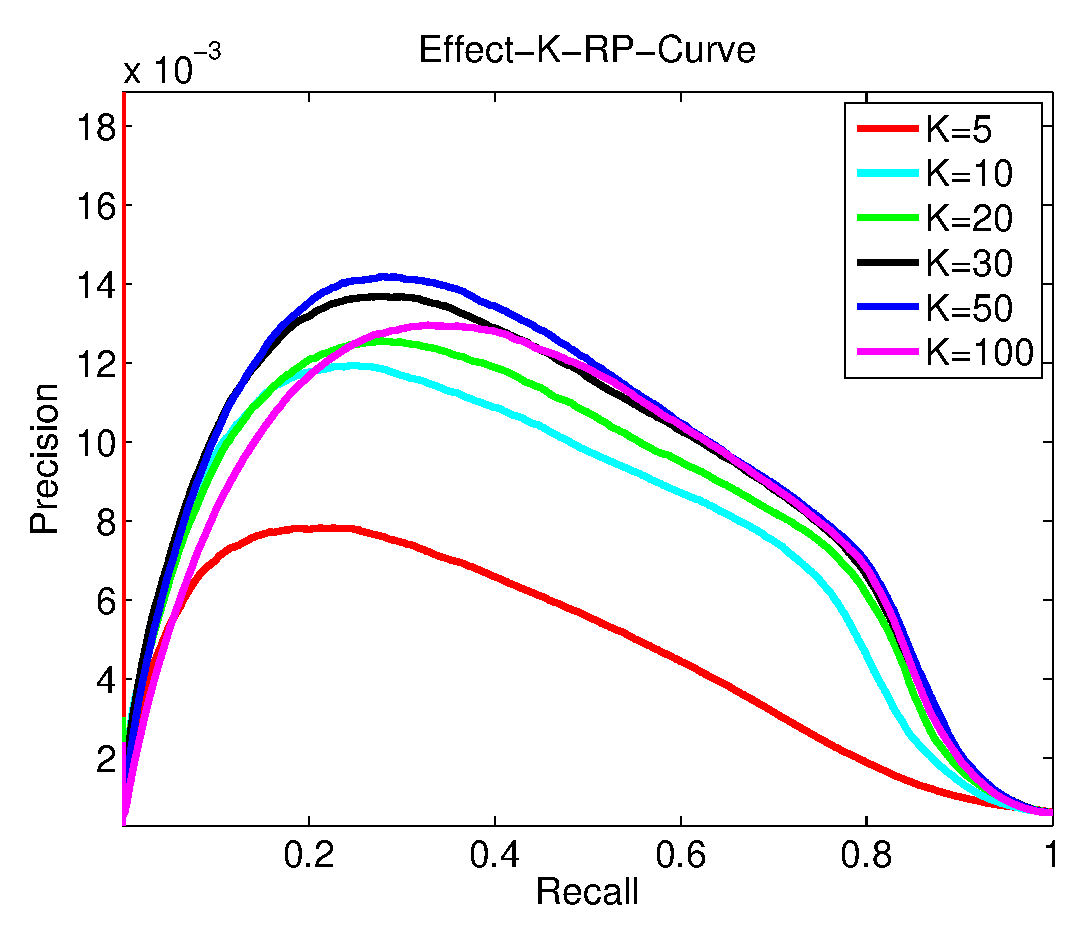
\includegraphics[width=65mm]{Effect_K/RP_Curve.eps}
    }
    \subfloat{
        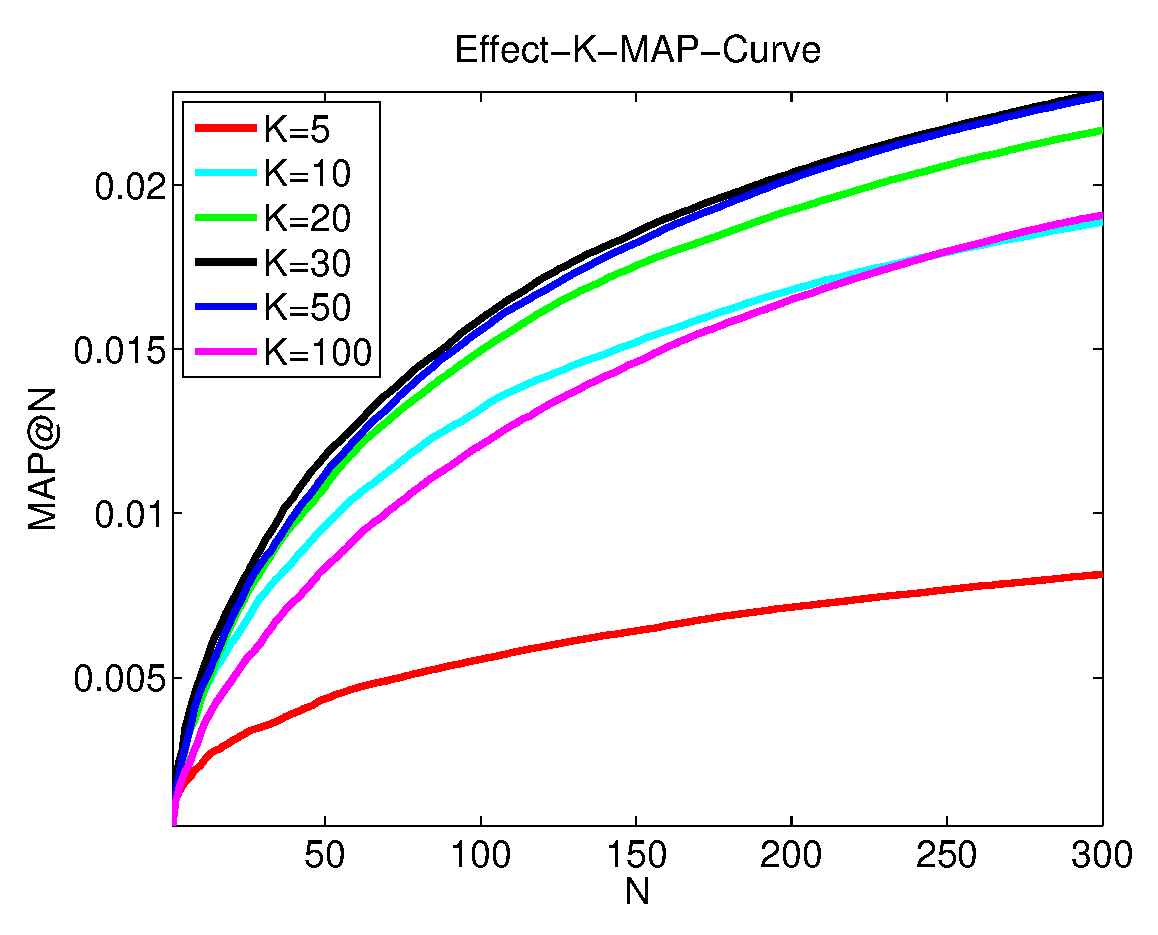
\includegraphics[width=70mm]{Effect_K/MAP_Curve.eps}
    }
    \caption{Performance Comparison between the trained models with various
        $K=5,10,20,30,50$.  Left: Precision-Recall Curve. Right: MAP@N Curve. }
    \label{EffectK:RP_MAP}
\end{figure}

\subsection{Effects of Bias Weight $\alpha$}

\subsection{Effects of Regularization Parameter $\lambda$}

\subsection{Effects of Early Stopping}


\section{Experiment III: Revisits Feature Engineering}
\subsection{Best-Tuned Setting}

\subsection{Principal Component analysis}


\section{Experiment IV: Pre-clustered Matrix Completion}

\subsection{Results}



\begin{figure}[h]

    \caption{Precision v.s. Recall Comparison between models with
        $\lambda=\lambda_0, \lambda_1,\lambda_2, \lambda_3$ }
\end{figure}

\begin{figure}[h]

    \caption{Precision v.s. Recall Comparison between various models with
        different preprocessed data}
\end{figure}

\section{Conclusions}
% one concluding paragraph
Features do provide supervision for recognizing the pattern of new users. 

% in the future
Future work can be extended to modeling time-series recommendation problem by
means of one-class inductive matrix completion. 

%\subsubsection*{References}
\bibliography{main}{}
\bibliographystyle{plain}


\end{document}
